% -*- mode: noweb; noweb-default-code-mode: R-mode; -*-
%\VignetteIndexEntry{cn.farms: Manual for the R package}
%\VignetteDepends{cn.farms}
%\VignettePackage{cn.farms}
%\VignetteKeywords{copy number analysis, factor analysis, sparse coding, latent variables, Laplace distribution, EM algorithm, microarray, farms, CNV, copy number}

\documentclass[article]{bioinf}

\usepackage{amsmath,amssymb}
\usepackage{bm}
\usepackage{natbib}
\usepackage{hyperref}

\usepackage{cnFarmsDefs}

\hypersetup{colorlinks=false,
   pdfborder=0 0 0,
   pdftitle={cn.FARMS: Manual for the R package},
   pdfauthor={Djork-Arn\'e Clevert and Andreas Mitterecker}}

\title{cn.FARMS: a latent variable model to detect copy
number variations in microarray data with a low false discovery rate \\ \textit{---
    Manual for the \Rpackage{cn.farms} package ---}}

\author{Djork-Arn\'e Clevert and Andreas Mitterecker}
\affiliation{Institute of Bioinformatics, Johannes Kepler University
Linz\\Altenberger Str. 69, 4040 Linz, Austria\\
\email{okko@clevert.de and mitterecker@bioinf.jku.at}}

\usepackage[noae]{Sweave}



\begin{document}


\newcommand{\farmsVers}{0.99.5}

\manualtitlepage[Version \farmsVers, \today]

\newlength{\auxparskip}
\setlength{\auxparskip}{\parskip}
\setlength{\parskip}{0pt}
\tableofcontents
\clearpage
\setlength{\parskip}{\auxparskip}
\section{Introduction}

The \Rpackage{cn.farms} package provides 
a novel copy number variation (CNV) detection method, called ``cn.FARMS'', 
which is based on our FARMS (``factor analysis for robust microarray
summarization'' \citep{Hochreiter:06}) algorithm. 
FARMS is since 2006 the leading summarization 
method of the international ``affycomp'' competition if sensitivity 
and specificity are considered simultaneously. 
We extended FARMS to cn.FARMS \citep{Clevert:11}
for detecting CNVs by moving from mRNA copy numbers to
DNA copy numbers.\\
In the following section we will briefly describe the algorithm and provide
a quick start guide.
For furhter information regarding the algorithm and its assessment 
see the \Rpackage{cn.farms} homepage at
\href{http://www.bioinf.jku.at/software/cnfarms/cnfarms.html}{http://www.bioinf.jku.at/software/cnfarms/cnfarms.html}.

\section{cn.FARMS: FARMS for CNV Detection}
\label{sec:farmspipeline}
cn.FARMS is described ``in a nutshell''  by the preprocessing pipeline depicted
in Figure \ref{fig:preprocess_chain_fig}:\linebreak
{\bf (1) Normalization} is performed at two levels.
It has as {\em input} the raw probe intensity values and
as {\em output} intensity values at chromosome locations
which are leveled between arrays and are allele independent.
At the {\em first level} normalization methods 
remove technical variations between arrays arising from 
differences in sample preparation or labeling, 
array production (e.g.\ batch effects), or scanning differences.
The goal of the first level is to correct for array-wide effects.
At the {\em second level} alleles are combined to one intensity
value at a chromosome location and a correction for
cross-hybridization between allele A and allele B probes is
performed.
Cross-hybridization arise due to close 
sequence similarity between the probes of different alleles, therefore a
probe of one allele picks up a signal of the other allele.
The optional corrections for differences in
PCR yield can be
performed at this step or after ``single-locus
modeling''.
\begin{figure}[!b]
\begin{center}
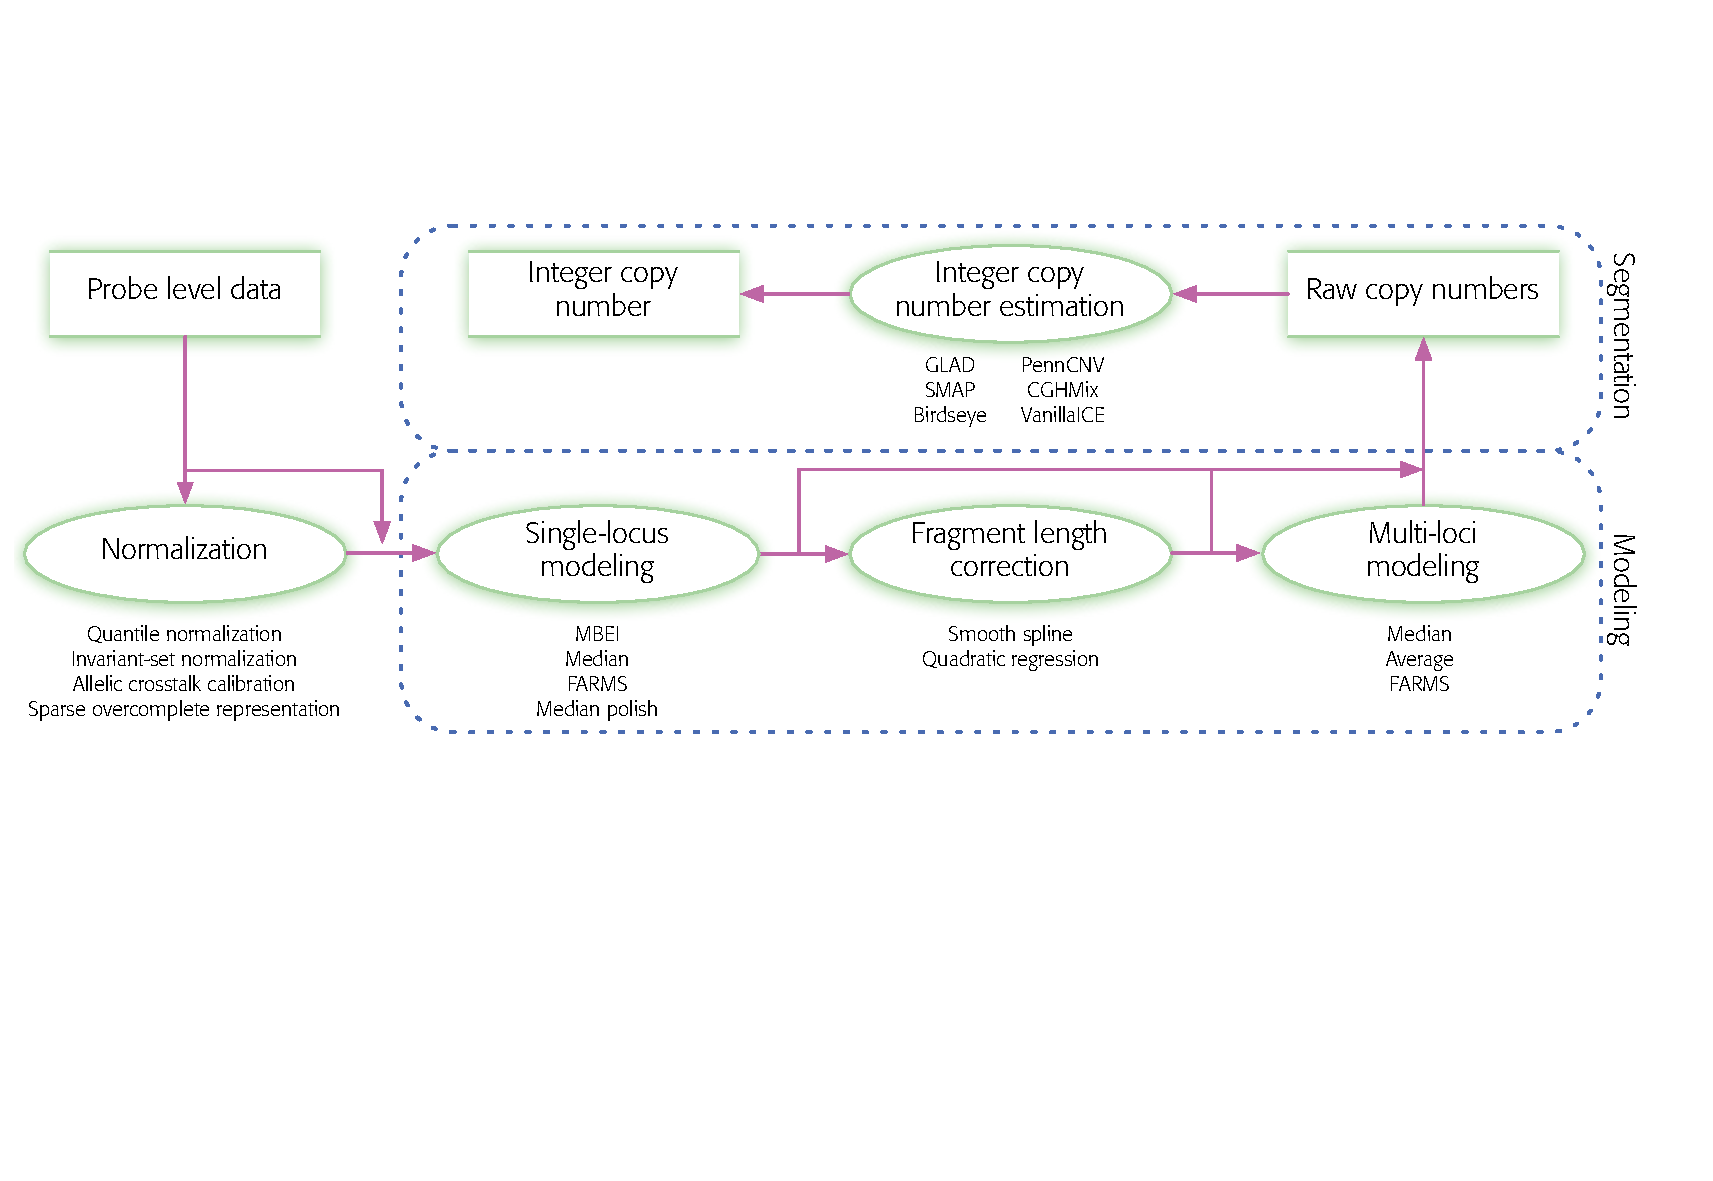
\includegraphics[angle=0,width=0.99\textwidth]{figures/figure2}
\caption{Copy number analysis for (Affymetrix) DNA genotyping arrays
as a three-step pipeline: (1) Normalization, (2) Modeling, and (3) Segmentation.
Modeling is divided into ``single-locus modeling'' and ``multi-loci
modeling'' with ``fragment length
correction'' as an optional intermediate step. 
The cn.FARMS pipeline is: normalization by sparse
overcomplete representation, single-locus modeling by FARMS, fragment length
correction, and multi-loci modeling by FARMS. 
\label{fig:preprocess_chain_fig}}
\end{center}
\end{figure} 
We propose sparse overcomplete representation in the two-dimensional 
space of allele A and B intensity to correct for cross-hybridization between 
allele A and allele B probes. Therefore we do not only estimate the AA and the BB
cross-hybridization like CRMA \citep{Bengtsson:08} but also the AB cross-hybridization. The
latter takes into account that hybridization and cross-hybridization
may be different for the AB genotype, where for both allele probes 
target fragments are available and compete for hybridization. 
After allele correction, we follow CRMA and normalize by scaling the probes
to a pre-specified mean intensity value. CNV probes which have only one
allele are scaled in the same way. \linebreak 
{\bf(2) Modeling} is also performed at two levels.
The {\em input} is the probe intensity values which 
independently measure the copy number of a specific target fragment or
DNA probe locus.
The {\em output} is an estimate for the region copy number.
At the {\em first level}, ``single-locus modeling'' the probes which
measure the same fragment are combined to a raw fragment copy number (``raw''
means that the copy number is still a continuous values) --- 
see Figure~\ref{fig:meta_probeset_fig}. These raw fragment
  copy numbers are estimated by FARMS. 
The original FARMS was designed to
summarize probes which target the same mRNA. This can readily
transfered to CNV analysis where FARMS now summarizes probes which
target the same DNA fragment. Either both strands can be
summarized together or separately where our default is the former.
\cite{Nannya:05} suggested considering
fragment characteristics  like sequence patterns and the length because
they affect PCR amplification.
For example, PCR is usually less efficient for  
longer fragments, which lead to fewer copies to hybridize and
result in weaker probe intensities.
Following these suggestions cn.FARMS performs an optional intermediate 
level to correct for the fragment length and sequence features to  
make raw fragment copy numbers comparable along the
chromosome.
At the {\em second level}, ``multi-loci modeling'', the raw copy numbers
of neighboring fragments or neighboring  DNA probe loci
are combined to a ``meta-probe set'' which
targets a DNA region. 
\begin{figure}[t]
\begin{center}
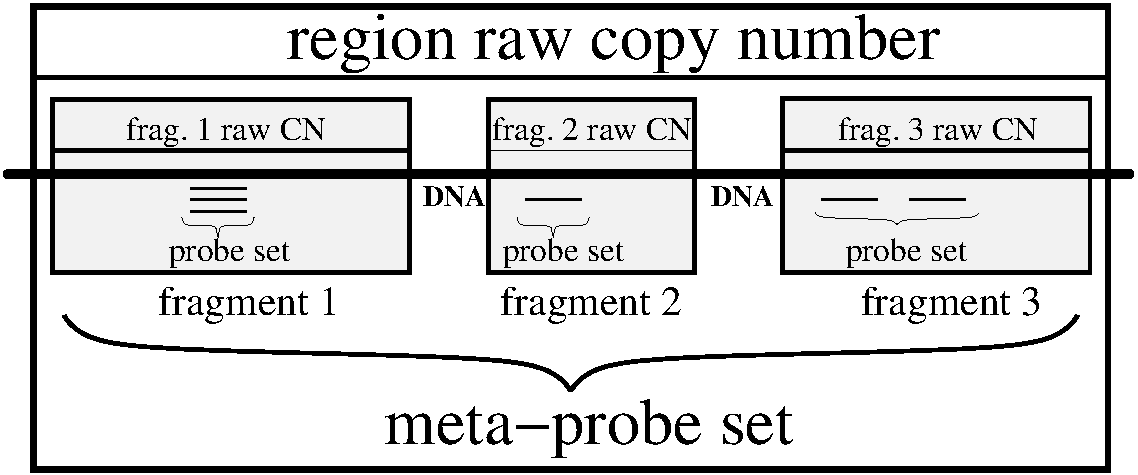
\includegraphics[angle=0,width= 0.75\columnwidth]{figures/figure1}
\caption{The copy number hierarchy
probes-fragment-region. Fragment copy numbers serve as  
meta-probes used for ``multi-loci modeling'' which yields region copy numbers.
Inner boxes: The probes which target a fragment (often at a SNP
  position) are single-locus summarized to a raw copy number of this fragment.
Note, that instead of fragments a DNA probe loci can be summarized. Outer box: The
  raw fragment copy numbers are the meta-probes for a DNA
  region and are multi-loci summarized to a raw region copy number.
\label{fig:meta_probeset_fig}}
\end{center}
\end{figure} 
The raw fragment copy numbers from single-locus modeling are now themselves
probes for a DNA region as depicted in Figure~\ref{fig:meta_probeset_fig}.
Again we use FARMS to summarize meta-probes and
to estimate a raw copy number for the region. This modeling across 
samples is novel as previous methods only model along the chromosome. 
Multi-loci modeling considerably reduces
the false discovery rates, because raw copy numbers of
neighboring fragments or neighboring DNA probe loci must agree to each other 
on the copy number, which reduces the likelihood of a discovery by chance.
However, low FDR is traded against high resolution by 
the window size for multi-loci modeling, i.e.~
by how many raw copy numbers of neighboring fragments or neighboring
DNA probe loci are combined. 
The more loci are combined, the more the FDR is reduced, because more  
meta-probes must mutually agree on the region's copy number.
The window size for multi-loci modeling is 
a hyperparameter which trades off low FDR against high resolution. 
We recommend a window size of 5 as default, 3 for high
resolution, and 10 for low FDR.
Alternatively to a fixed number of CNV or
SNP sites, the cn.FARMS software allows defining a window in terms of base pairs.
In this case, multi-loci modeling may use a different number
of meta-probes at different DNA locations, in particular for less than
two meta-probes multi-loci modeling is skipped. 
Note, however that controlling the FDR is more
difficult because a minimal number of meta-probes cannot be assured
for each window and modeling with few meta-probes is prone to false discoveries.
FARMS supplies an informative/non-informative (I/NI) call \citep{Talloen:07,Talloen:10}
which is used to detect CNVs. Additionally, the I/NI value  gives the
signal-to-noise-ratio of the estimated raw copy number.\linebreak
{\bf(3) Segmentation} can afterwards be performed by  \Rpackage{DNAcopy}.







\section{Getting Started: cn.FARMS}
\label{sec:started}

As usual, it is necessary to load the \Rpackage{cn.farms} package:
\begin{Sinput}
library(cn.farms)
\end{Sinput}

\subsection{Quick start : Process SNP 6.0 array}

\noindent The \Rpackage{hapmapsnp6} package is loaded for testing purpose.

\begin{Sinput}
> library("hapmapsnp6") 
> celDir <- system.file("celFiles", package="hapmapsnp6")
> filenames <- dir(path=celDir, full.names=TRUE)
\end{Sinput}

\noindent  Next, the user specifies a working directory on the harddisk whereto save the results.

\begin{Sinput}
> workDir <- "~/tmp"
> dir.create(workDir, showWarnings=F, recursive=T)
> setwd(workDir)
\end{Sinput}

\noindent For reasons of computational time and memory consumption \Rpackage{cn.farms} supports high-performance computation. 
The parameter  \verb+cores+ specifies number amount of CPUs requested for the cluster and  the parameter  \verb+runtype+
indicates how the data matrix should be stored.   \verb+runtype = "ff"+ creates a transient flat-file which will not be saved automatically.
Whereas  \verb+runtype = "bm"+ creates a persistent flat-file which can be save permanently.

\begin{Sinput}
> cores <- 2
> runtype <- "bm"
\end{Sinput}

\noindent  Next, the user specifies a subdirectory whereto save the flat-files.

\begin{Sinput}
> dir.create("ffObjects/ff", showWarnings=F, recursive=T)
> oligoClasses::ldPath(file.path(getwd(), "ffObjects"))
> options(fftempdir = file.path(oligoClasses::ldPath(), "ff"))
\end{Sinput}

\noindent  The directory (\verb+celDir = "where/are/my/cel-files"+) which contain the cel-files has to be specified. 

\begin{Sinput}
> celDir <- system.file("celFiles", package="hapmapsnp6")
> filenames <- dir(path=celDir, full.names=TRUE)
\end{Sinput}

\noindent The following step will create the annotation file.

\begin{Sinput}
> if(exists("annotDir")) {
>	createAnnotation(filenames=filenames, annotDir=annotDir)	
> } else {
> 	createAnnotation(filenames=filenames)
> }
\end{Sinput}

\noindent Afterwards, the data will be corrected for cross-hybridization and normalized.

\begin{Sinput}
> normMethod <- "SOR"

> ## normalization of SNP data
> if(exists("annotDir")) {
> 	normData <- normalizeCels(filenames, method=normMethod, cores, alleles=T, 
> 			annotDir=annotDir, runtype=runtype)
> } else {
> 	normData <- normalizeCels(filenames, method=normMethod, cores, alleles=T, 
> 			runtype=runtype)
> }
\end{Sinput}

\noindent Now, the normalized data will be summarized at DNA probe loci. \verb+summaryMethod <-  "Variational"+ indicates which FARMS
approach should be used and \verb+summaryParam$cyc <- c(10, 10)+ specifies the number of iterations of the EM-algorithm. The parameter 
\verb+summaryWindow+ indicates whether DNA probe loci on the same DNA fragments are summarized together (\verb+summaryWindow="fragment"+) 
or if the DNA probe loci are summarized separately (\verb+summaryWindow="std"+ is the default setting).


\begin{Schunk}
\begin{Sinput}
> summaryMethod <- "Variational"
> summaryParam <- list()
> summaryParam$cyc <- c(10)
> callParam <- list(cores = cores, runtype = runtype)
> slData <- slSummarization(normData, summaryMethod = summaryMethod, 
+     summaryParam = summaryParam, callParam = callParam, summaryWindow = "std")
\end{Sinput}
\begin{Soutput}
2011-04-05 10:05:08 |   Starting summarization 
2011-04-05 10:05:08 |   Computations will take some time, please be patient 
R Version:  R version 2.13.0 Under development (unstable) (2010-12-21 r53879) 

2011-04-05 10:05:13 |   Summarizing batch 1 ... 
2011-04-05 10:05:15 |   Summarization done 
Time difference of 7.390061 secs
\end{Soutput}
\begin{Sinput}
> show(slData)
\end{Sinput}
\begin{Soutput}
ExpressionSet (storageMode: list)
assayData: 319 features, 3 samples 
  element names: intensity, L_z, INICall, IC, lapla 
protocolData: none
phenoData
  rowNames: NA06985_GW6_C NA06991_GW6_C NA06993_GW6_C
  varLabels: filenames batch gender
  varMetadata: labelDescription
featureData
  featureNames: 906474 745070 ... 888581 (319 total)
  fvarLabels: chrom start ... fragment_length2 (10 total)
  fvarMetadata: labelDescription
experimentData: use 'experimentData(object)'
Annotation: pd.genomewidesnp.6 
\end{Soutput}
\begin{Sinput}
> assayData(slData)$intensity[1:10, ]
\end{Sinput}
\begin{Soutput}
          [,1]     [,2]     [,3]
 [1,] 12.20755 12.17502 12.32406
 [2,] 10.11318 10.37334 10.28581
 [3,] 10.63524 10.67435 10.67910
 [4,] 11.97147 11.86901 12.19888
 [5,] 11.35531 11.64151 11.57714
 [6,] 11.80594 11.69453 11.88172
 [7,] 10.83750 11.30031 11.52272
 [8,] 11.15025 11.61968 11.34616
 [9,] 11.79847 11.79846 11.79846
[10,] 11.65713 12.14412 12.42084
\end{Soutput}
\begin{Sinput}
> assayData(slData)$L_z[1:10, ]
\end{Sinput}
\begin{Soutput}
               [,1]         [,2]          [,3]
 [1,] -7.517762e-03 -0.040046276  1.089872e-01
 [2,] -1.705384e-01  0.089626390  2.094587e-03
 [3,] -3.764501e-02  0.001457699  6.213158e-03
 [4,] -4.024762e-04 -0.102867004  2.270022e-01
 [5,] -2.218426e-01  0.064355342 -1.436268e-05
 [6,]  3.354704e-05 -0.111374832  7.581430e-02
 [7,] -4.616970e-01  0.001114454  2.235242e-01
 [8,] -1.983893e-01  0.271041282 -2.482165e-03
 [9,]  7.178394e-06  0.000000000 -3.878486e-06
[10,] -4.869916e-01  0.000000000  2.767239e-01
\end{Soutput}
\end{Schunk}


\noindent Now, the intensity values of the non-polymorphic probes (CN-probes) were normalized.

\begin{Sinput}
> if (exists("annotDir")) {
	npData <- normalizeNpData(filenames, cores, annotDir=annotDir)	
 } else {
	npData <- normalizeNpData(filenames, cores, runtype=runtype)
 }
\end{Sinput}

\noindent This step combines non-polymorphic probes and single-locus summarized SNP-probes.

\begin{Schunk}
\begin{Sinput}
> combData <- combineData(slData, npData, runtype = runtype)
> show(combData)
\end{Sinput}
\begin{Soutput}
ExpressionSet (storageMode: list)
assayData: 638 features, 3 samples 
  element names: intensity 
protocolData: none
phenoData
  rowNames: NA06985_GW6_C NA06991_GW6_C NA06993_GW6_C
  varLabels: filenames batch gender
  varMetadata: labelDescription
featureData
  featureNames: 906474 9064741 ... 8885811 (638 total)
  fvarLabels: chrom start end man_fsetid
  fvarMetadata: labelDescription
experimentData: use 'experimentData(object)'
Annotation: pd.genomewidesnp.6 
\end{Soutput}
\end{Schunk}

\noindent In this final step intensity values of non-polymorphic probes and single-locus 
summarized SNP-probes are multi-locus summarized with a windows size of 5 probes  (\verb+windowParam$windowSize <- 5+).
The window size for multi-loci modeling is 
a hyperparameter which trades off low FDR against high resolution. 
We recommend a window size of 5 as default, 3 for high
resolution, and 7 for low FDR. Setting \verb+windowParam$overlap <- TRUE+ inidicates that
the multi-locus summariaztion is done by step-wise moving the window over the genome. 
Alternatively to a fixed number of CNV or
SNP sites, the cn.FARMS software allows defining a window in terms of base pairs. To make 
use of this option set \verb+windowMethod <- "bps"+. 
In this case, multi-loci modeling may use a different number
of meta-probes at different DNA locations, in particular for less than
two meta-probes multi-loci modeling is skipped. 
Note, however that controlling the FDR is more
difficult because a minimal number of meta-probes cannot be assured
for each window and modeling with few meta-probes is prone to false discoveries.


\begin{Schunk}
\begin{Sinput}
> windowMethod <- "std"
> windowParam <- list()
> windowParam$windowSize <- 5
> windowParam$overlap <- TRUE
> summaryMethod <- "Variational"
> summaryParam <- list()
> summaryParam$cyc <- c(20)
> callParam <- list(cores = cores, runtype = runtype)
> mlData <- mlSummarization(slData, windowMethod = windowMethod, 
+     windowParam = windowParam, summaryMethod = summaryMethod, 
+     summaryParam = summaryParam, callParam = callParam)
\end{Sinput}
\begin{Soutput}
2011-04-05 10:05:16 |   Starting summarization 
2011-04-05 10:05:16 |   Computations will take some time, please be patient 
2011-04-05 10:05:22 |   Summarizing batch 1 ... 
2011-04-05 10:05:23 |   Summarization done 
\end{Soutput}
\begin{Sinput}
> assayData(mlData)
\end{Sinput}
\begin{Soutput}
$intensity
ff (open) double length=945 (945) dim=c(315,3) dimorder=c(1,2)
           [,1]     [,2]     [,3]
[1,]   11.25614 11.36881 11.34344
[2,]   11.17581 11.28848 11.26311
[3,]   11.31831 11.46689 11.48400
[4,]   11.43798 11.64570 11.60267
[5,]   11.56560 11.56560 11.56560
[6,]   11.67900 11.67900 11.67900
[7,]   11.75993 11.75994 11.75994
[8,]   11.98562 11.98562 11.98562
:             :        :        :
[308,] 12.45345 12.36589 12.57690
[309,] 12.63058 12.54857 12.73486
[310,] 12.37031 12.31327 12.43549
[311,] 12.50302 12.36214 12.54567
[312,] 12.37075 12.21500 12.37619
[313,] 12.38909 12.23160 12.43595
[314,] 12.17181 12.17181 12.17181
[315,] 12.46419 12.46419 12.46419

$L_z
ff (open) double length=945 (945) dim=c(315,3) dimorder=c(1,2)
                [,1]          [,2]          [,3]
[1,]   -8.712036e-02  2.554806e-02  1.771981e-04
[2,]   -8.713133e-02  2.554272e-02  1.720637e-04
[3,]   -1.475322e-01  1.048626e-03  1.815850e-02
[4,]   -1.622197e-01  4.549467e-02  2.469572e-03
[5,]   -4.772754e-07  2.053982e-07  8.198186e-08
[6,]   -2.405087e-07  6.353837e-08  1.026209e-07
[7,]   -2.532603e-06  3.560109e-07  1.486818e-06
[8,]   -4.093355e-11 -9.282559e-11  1.374473e-10
:                  :             :             :
[308,] -1.365211e-05 -8.758209e-02  1.234337e-01
[309,] -3.249869e-06 -8.201717e-02  1.042746e-01
[310,] -1.612020e-04 -5.719566e-02  6.501597e-02
[311,] -3.235122e-05 -1.409128e-01  4.261905e-02
[312,] -3.011554e-07 -1.557494e-01  5.439266e-03
[313,] -6.016888e-05 -1.575518e-01  4.680149e-02
[314,] -4.343949e-14 -6.959897e-13  1.294788e-13
[315,]  0.000000e+00 -2.302694e-09  1.053619e-09

$INICall
ff (open) double length=315 (315) dim=c(315,1) dimorder=c(1,2)
               [,1]
[1,]   1.523963e-01
[2,]   1.524092e-01
[3,]   1.796878e-01
[4,]   1.900381e-01
[5,]   2.239515e-12
[6,]   4.782716e-13
[7,]   6.163425e-11
[8,]   0.000000e+00
:                 :
[308,] 1.241166e-01
[309,] 1.243723e-01
[310,] 1.119241e-01
[311,] 1.127761e-01
[312,] 1.095954e-01
[313,] 1.087332e-01
[314,] 0.000000e+00
[315,] 0.000000e+00

$IC
ff (open) double length=945 (945) dim=c(315,3) dimorder=c(1,2)
              [,1]        [,2]        [,3]
[1,]     5.6682722   5.6593622  -1.4422158
[2,]     5.7116205   5.7029681  -1.4407859
[3,]     5.0689252   0.9523697   4.9911356
[4,]     3.1157307   3.0460854  -1.0574463
[5,]    -2.7825724  -3.6766874  -5.6732631
[6,]    -2.2851859  -4.1516919  -3.2054672
[7,]    -2.3131709  -5.8497754  -2.8056725
[8,]   -16.7660839 -15.2916332 -14.9079047
:                :           :           :
[308,] -10.8474429   5.3582017   5.3595555
[309,] -11.0885036   7.1354541   7.1357227
[310,]  -6.3387786   3.1714310   3.1734243
[311,]  -9.4629885   4.5953200   4.5820613
[312,] -16.0794333   7.9579910   7.8831565
[313,]  -9.7776991   3.6691009   3.6439874
[314,] -30.1954206 -24.9145587 -27.2740543
[315,]        -Inf  -3.4968829  -4.2837363

$lapla
ff (open) double length=945 (945) dim=c(315,3) dimorder=c(1,2)
               [,1]         [,2]         [,3]
[1,]   1.527427e-01 1.518023e-01 1.105326e-03
[2,]   1.527454e-01 1.518321e-01 1.073691e-03
[3,]   1.804455e-01 1.040254e-02 1.709736e-01
[4,]   1.932613e-01 1.841533e-01 1.071256e-02
[5,]   1.453323e-01 7.820001e-02 1.959646e-02
[6,]   2.051590e-01 5.626213e-02 1.084072e-01
[7,]   2.012177e-01 1.733972e-02 1.430238e-01
[8,]   8.972343e-06 2.493215e-05 3.252921e-05
:                 :            :            :
[308,] 1.643938e-06 1.242426e-01 1.243593e-01
[309,] 4.063703e-07 1.244171e-01 1.244402e-01
[310,] 1.544024e-04 1.125933e-01 1.127490e-01
[311,] 6.634377e-06 1.131808e-01 1.121454e-01
[312,] 6.367406e-09 1.096348e-01 1.040928e-01
[313,] 9.802667e-06 1.094547e-01 1.075659e-01
[314,] 8.133410e-10 3.162063e-08 6.161572e-09
[315,] 0.000000e+00 8.857952e-02 5.134130e-02
\end{Soutput}
\end{Schunk}

\noindent Next, the summarized data will be segmented in order to identify break points. Therefore we provide a parallelized version of
\Rpackage{DNAcopy}. 


\begin{Schunk}
\begin{Sinput}
> colnames(assayData(mlData)$L_z) <- sampleNames(mlData)
> segments <- dnaCopySf(x = assayData(mlData)$L_z, chrom = featureData(mlData)@data$chrom, 
+     maploc = featureData(mlData)@data$start, cores = cores, 
+     smoothing = FALSE)
\end{Sinput}
\begin{Soutput}
Library ff loaded.
Library DNAcopy loaded.
Time difference of 7.25407 secs
\end{Soutput}
\begin{Sinput}
> featureData(segments)@data
\end{Sinput}
\begin{Soutput}
   chrom   start     end num.mark seg.mean    individual
1      1  564621  752566        4  -0.1210 NA06985_GW6_C
2      1  761732 2456203      153  -0.0054 NA06985_GW6_C
3      1 2473258 2553624        9   0.2969 NA06985_GW6_C
4      1 2553758 2766971       12  -0.0149 NA06985_GW6_C
5      1 2783040 2787707        3   0.1621 NA06985_GW6_C
6      1 2789108 2859724       17  -0.0071 NA06985_GW6_C
7      1 2865778 2867961        4  -0.1951 NA06985_GW6_C
8      1 2878366 2925522       13   0.0006 NA06985_GW6_C
9      1 2926555 2936480        5  -0.0632 NA06985_GW6_C
10     1 2936870 2974212       16  -0.0008 NA06985_GW6_C
11     1 2981841 2996602        5  -0.1455 NA06985_GW6_C
12     1 3000924 3025712        6   0.0005 NA06985_GW6_C
13     1 3026100 3044181        3   0.2138 NA06985_GW6_C
14     1 3044977 3080940       10  -0.0037 NA06985_GW6_C
15     1 3089849 3101863        6  -0.2318 NA06985_GW6_C
16     1 3103312 3112417        4  -0.0923 NA06985_GW6_C
17     1 3112979 3225940       45   0.0001 NA06985_GW6_C
18     1  564621 1871337       75  -0.0164 NA06991_GW6_C
19     1 1888193 1948400        5  -0.4476 NA06991_GW6_C
20     1 1972462 2996602      161  -0.0239 NA06991_GW6_C
21     1 3000924 3047252       11  -0.1100 NA06991_GW6_C
22     1 3049713 3220101       54  -0.0043 NA06991_GW6_C
23     1 3220160 3225940        9  -0.0852 NA06991_GW6_C
24     1  564621  792480        9   0.0112 NA06993_GW6_C
25     1  798959 1003629       11   0.1959 NA06993_GW6_C
26     1 1017216 1218086       20   0.0661 NA06993_GW6_C
27     1 1242215 1365570        8   0.1774 NA06993_GW6_C
28     1 1411876 1500941        7   0.0000 NA06993_GW6_C
29     1 1506035 1663831        4   0.1057 NA06993_GW6_C
30     1 1688192 2285414       66   0.0151 NA06993_GW6_C
31     1 2286408 2302911        4   0.1805 NA06993_GW6_C
32     1 2303512 2329564       11   0.0000 NA06993_GW6_C
33     1 2329661 2455633       15   0.0660 NA06993_GW6_C
34     1 2455863 2553758       12   0.0048 NA06993_GW6_C
35     1 2701816 2723345        3   0.1696 NA06993_GW6_C
36     1 2723552 2833332       20   0.0043 NA06993_GW6_C
37     1 2833743 2846274        5   0.1422 NA06993_GW6_C
38     1 2851238 2932446       23   0.0204 NA06993_GW6_C
39     1 2934312 2950334        9   0.1407 NA06993_GW6_C
40     1 2950370 3050594       27   0.0336 NA06993_GW6_C
41     1 3054106 3089849        7   0.1476 NA06993_GW6_C
42     1 3094831 3114952       11   0.0645 NA06993_GW6_C
43     1 3119489 3127925        7   0.1607 NA06993_GW6_C
44     1 3135175 3152968       11   0.0071 NA06993_GW6_C
45     1 3165267 3197480        6   0.1902 NA06993_GW6_C
46     1 3197747 3225940       19   0.0436 NA06993_GW6_C
\end{Soutput}
\end{Schunk}

\noindent To get further information, e.g. how to process Affymetrix 500K arrays, please check the followings demos.  

\begin{Sinput}
> demo(package = "cn.farms")

Demos in package 'cn.farms':

demo01Snp6            Demo for an Affymetrix SNP6 data set
demo02Snp5            Demo for an Affymetrix SNP5 data set
demo03Snp500k         Demo for an Affymetrix 500K data set
demo04Snp250k         Demo for an Affymetrix 250K NSP data set
demo05Testing         Run the examples
\end{Sinput}

\section{Setup}
\label{sec:setup}

This vignette was built on:
\begin{Schunk}
\begin{Sinput}
> sessionInfo()
\end{Sinput}
\begin{Soutput}
R version 2.13.0 Under development (unstable) (2010-12-21 r53879)
Platform: x86_64-unknown-linux-gnu (64-bit)

locale:
 [1] LC_CTYPE=en_US.UTF-8       LC_NUMERIC=C              
 [3] LC_TIME=en_US.UTF-8        LC_COLLATE=en_US.UTF-8    
 [5] LC_MONETARY=C              LC_MESSAGES=en_US.UTF-8   
 [7] LC_PAPER=en_US.UTF-8       LC_NAME=C                 
 [9] LC_ADDRESS=C               LC_TELEPHONE=C            
[11] LC_MEASUREMENT=en_US.UTF-8 LC_IDENTIFICATION=C       

attached base packages:
[1] tools     stats     graphics  grDevices utils     datasets  methods  
[8] base     

other attached packages:
[1] DNAcopy_1.25.0  snow_0.3-3      cn.farms_0.99.5 ff_2.2-1       
[5] bit_1.1-6       Biobase_2.11.8 

loaded via a namespace (and not attached):
 [1] affxparser_1.23.1     affyio_1.19.3         Biostrings_2.19.8    
 [4] DBI_0.2-5             grid_2.13.0           IRanges_1.9.21       
 [7] lattice_0.19-17       oligo_1.15.2          oligoClasses_1.13.9  
[10] preprocessCore_1.13.5 snowfall_1.84         splines_2.13.0       
\end{Soutput}
\end{Schunk}


\bibliographystyle{natbib}
\bibliography{cnv}

\end{document}
